\documentclass[1p]{elsarticle_modified}
%\bibliographystyle{elsarticle-num}

%\usepackage[colorlinks]{hyperref}
%\usepackage{abbrmath_seonhwa} %\Abb, \Ascr, \Acal ,\Abf, \Afrak
\usepackage{amsfonts}
\usepackage{amssymb}
\usepackage{amsmath}
\usepackage{amsthm}
\usepackage{scalefnt}
\usepackage{amsbsy}
\usepackage{kotex}
\usepackage{caption}
\usepackage{subfig}
\usepackage{color}
\usepackage{graphicx}
\usepackage{xcolor} %% white, black, red, green, blue, cyan, magenta, yellow
\usepackage{float}
\usepackage{setspace}
\usepackage{hyperref}

\usepackage{tikz}
\usetikzlibrary{arrows}

\usepackage{multirow}
\usepackage{array} % fixed length table
\usepackage{hhline}

%%%%%%%%%%%%%%%%%%%%%
\makeatletter
\renewcommand*\env@matrix[1][\arraystretch]{%
	\edef\arraystretch{#1}%
	\hskip -\arraycolsep
	\let\@ifnextchar\new@ifnextchar
	\array{*\c@MaxMatrixCols c}}
\makeatother %https://tex.stackexchange.com/questions/14071/how-can-i-increase-the-line-spacing-in-a-matrix
%%%%%%%%%%%%%%%

\usepackage[normalem]{ulem}

\newcommand{\msout}[1]{\ifmmode\text{\sout{\ensuremath{#1}}}\else\sout{#1}\fi}
%SOURCE: \msout is \stkout macro in https://tex.stackexchange.com/questions/20609/strikeout-in-math-mode

\newcommand{\cancel}[1]{
	\ifmmode
	{\color{red}\msout{#1}}
	\else
	{\color{red}\sout{#1}}
	\fi
}

\newcommand{\add}[1]{
	{\color{blue}\uwave{#1}}
}

\newcommand{\replace}[2]{
	\ifmmode
	{\color{red}\msout{#1}}{\color{blue}\uwave{#2}}
	\else
	{\color{red}\sout{#1}}{\color{blue}\uwave{#2}}
	\fi
}

\newcommand{\Sol}{\mathcal{S}} %segment
\newcommand{\D}{D} %diagram
\newcommand{\A}{\mathcal{A}} %arc


%%%%%%%%%%%%%%%%%%%%%%%%%%%%%5 test

\def\sl{\operatorname{\textup{SL}}(2,\Cbb)}
\def\psl{\operatorname{\textup{PSL}}(2,\Cbb)}
\def\quan{\mkern 1mu \triangleright \mkern 1mu}

\theoremstyle{definition}
\newtheorem{thm}{Theorem}[section]
\newtheorem{prop}[thm]{Proposition}
\newtheorem{lem}[thm]{Lemma}
\newtheorem{ques}[thm]{Question}
\newtheorem{cor}[thm]{Corollary}
\newtheorem{defn}[thm]{Definition}
\newtheorem{exam}[thm]{Example}
\newtheorem{rmk}[thm]{Remark}
\newtheorem{alg}[thm]{Algorithm}

\newcommand{\I}{\sqrt{-1}}
\begin{document}

%\begin{frontmatter}
%
%\title{Boundary parabolic representations of knots up to 8 crossings}
%
%%% Group authors per affiliation:
%\author{Yunhi Cho} 
%\address{Department of Mathematics, University of Seoul, Seoul, Korea}
%\ead{yhcho@uos.ac.kr}
%
%
%\author{Seonhwa Kim} %\fnref{s_kim}}
%\address{Center for Geometry and Physics, Institute for Basic Science, Pohang, 37673, Korea}
%\ead{ryeona17@ibs.re.kr}
%
%\author{Hyuk Kim}
%\address{Department of Mathematical Sciences, Seoul National University, Seoul 08826, Korea}
%\ead{hyukkim@snu.ac.kr}
%
%\author{Seokbeom Yoon}
%\address{Department of Mathematical Sciences, Seoul National University, Seoul, 08826,  Korea}
%\ead{sbyoon15@snu.ac.kr}
%
%\begin{abstract}
%We find all boundary parabolic representation of knots up to 8 crossings.
%
%\end{abstract}
%\begin{keyword}
%    \MSC[2010] 57M25 
%\end{keyword}
%
%\end{frontmatter}

%\linenumbers
%\tableofcontents
%
\newcommand\colored[1]{\textcolor{white}{\rule[-0.35ex]{0.8em}{1.4ex}}\kern-0.8em\color{red} #1}%
%\newcommand\colored[1]{\textcolor{white}{ #1}\kern-2.17ex	\textcolor{white}{ #1}\kern-1.81ex	\textcolor{white}{ #1}\kern-2.15ex\color{red}#1	}

{\Large $\underline{12a_{0391}~(K12a_{0391})}$}

\setlength{\tabcolsep}{10pt}
\renewcommand{\arraystretch}{1.6}
\vspace{1cm}\begin{tabular}{m{100pt}>{\centering\arraybackslash}m{274pt}}
\multirow{5}{120pt}{
	\centering
	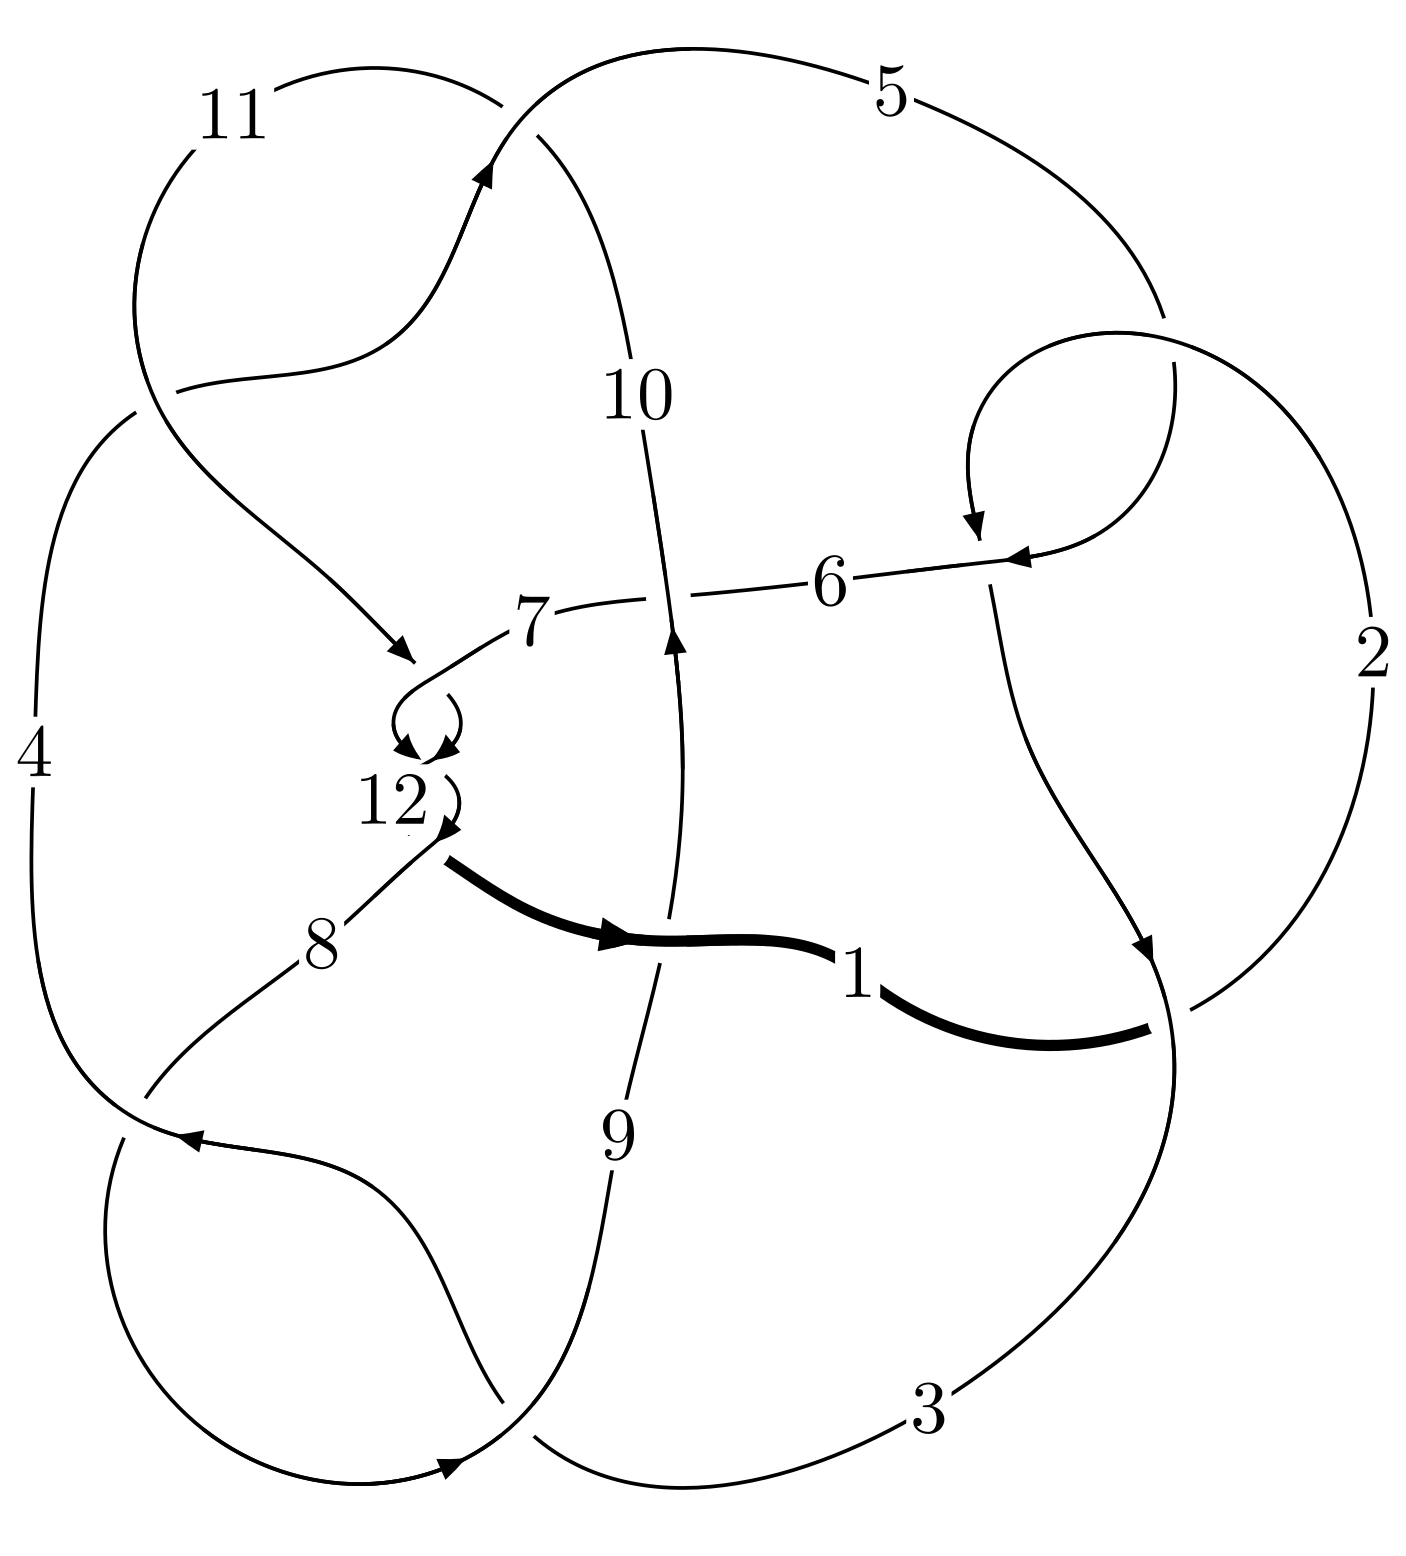
\includegraphics[width=112pt]{../../../GIT/diagram.site/Diagrams/png/1192_12a_0391.png}\\
\ \ \ A knot diagram\footnotemark}&
\allowdisplaybreaks
\textbf{Linearized knot diagam} \\
\cline{2-2}
 &
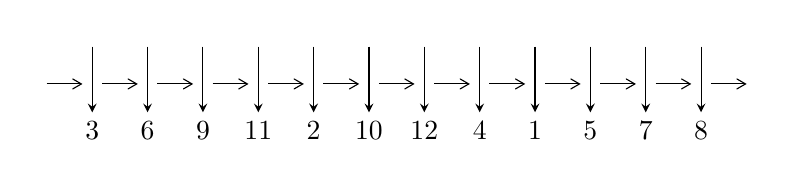
\begin{tikzpicture}[x=20pt, y=17pt]
	% nodes
	\node (C0) at (0, 0) {};
	\node (C1) at (1, 0) {};
	\node (C1U) at (1, +1) {};
	\node (C1D) at (1, -1) {3};

	\node (C2) at (2, 0) {};
	\node (C2U) at (2, +1) {};
	\node (C2D) at (2, -1) {6};

	\node (C3) at (3, 0) {};
	\node (C3U) at (3, +1) {};
	\node (C3D) at (3, -1) {9};

	\node (C4) at (4, 0) {};
	\node (C4U) at (4, +1) {};
	\node (C4D) at (4, -1) {11};

	\node (C5) at (5, 0) {};
	\node (C5U) at (5, +1) {};
	\node (C5D) at (5, -1) {2};

	\node (C6) at (6, 0) {};
	\node (C6U) at (6, +1) {};
	\node (C6D) at (6, -1) {10};

	\node (C7) at (7, 0) {};
	\node (C7U) at (7, +1) {};
	\node (C7D) at (7, -1) {12};

	\node (C8) at (8, 0) {};
	\node (C8U) at (8, +1) {};
	\node (C8D) at (8, -1) {4};

	\node (C9) at (9, 0) {};
	\node (C9U) at (9, +1) {};
	\node (C9D) at (9, -1) {1};

	\node (C10) at (10, 0) {};
	\node (C10U) at (10, +1) {};
	\node (C10D) at (10, -1) {5};

	\node (C11) at (11, 0) {};
	\node (C11U) at (11, +1) {};
	\node (C11D) at (11, -1) {7};

	\node (C12) at (12, 0) {};
	\node (C12U) at (12, +1) {};
	\node (C12D) at (12, -1) {8};
	\node (C13) at (13, 0) {};

	% arrows
	\draw[->,>={angle 60}]
	(C0) edge (C1) (C1) edge (C2) (C2) edge (C3) (C3) edge (C4) (C4) edge (C5) (C5) edge (C6) (C6) edge (C7) (C7) edge (C8) (C8) edge (C9) (C9) edge (C10) (C10) edge (C11) (C11) edge (C12) (C12) edge (C13) ;	\draw[->,>=stealth]
	(C1U) edge (C1D) (C2U) edge (C2D) (C3U) edge (C3D) (C4U) edge (C4D) (C5U) edge (C5D) (C6U) edge (C6D) (C7U) edge (C7D) (C8U) edge (C8D) (C9U) edge (C9D) (C10U) edge (C10D) (C11U) edge (C11D) (C12U) edge (C12D) ;
	\end{tikzpicture} \\
\hhline{~~} \\& 
\textbf{Solving Sequence} \\ \cline{2-2} 
 &
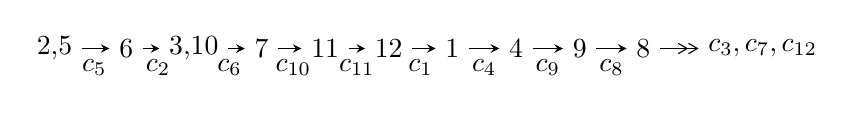
\begin{tikzpicture}[x=23pt, y=7pt]
	% node
	\node (A0) at (-1/8, 0) {2,5};
	\node (A1) at (1, 0) {6};
	\node (A2) at (33/16, 0) {3,10};
	\node (A3) at (25/8, 0) {7};
	\node (A4) at (33/8, 0) {11};
	\node (A5) at (41/8, 0) {12};
	\node (A6) at (49/8, 0) {1};
	\node (A7) at (57/8, 0) {4};
	\node (A8) at (65/8, 0) {9};
	\node (A9) at (73/8, 0) {8};
	\node (C1) at (1/2, -1) {$c_{5}$};
	\node (C2) at (3/2, -1) {$c_{2}$};
	\node (C3) at (21/8, -1) {$c_{6}$};
	\node (C4) at (29/8, -1) {$c_{10}$};
	\node (C5) at (37/8, -1) {$c_{11}$};
	\node (C6) at (45/8, -1) {$c_{1}$};
	\node (C7) at (53/8, -1) {$c_{4}$};
	\node (C8) at (61/8, -1) {$c_{9}$};
	\node (C9) at (69/8, -1) {$c_{8}$};
	\node (A10) at (11, 0) {$c_{3},c_{7},c_{12}$};

	% edge
	\draw[->,>=stealth]	
	(A0) edge (A1) (A1) edge (A2) (A2) edge (A3) (A3) edge (A4) (A4) edge (A5) (A5) edge (A6) (A6) edge (A7) (A7) edge (A8) (A8) edge (A9) ;
	\draw[->>,>={angle 60}]	
	(A9) edge (A10);
\end{tikzpicture} \\ 

\end{tabular} \\

\footnotetext{
The image of knot diagram is generated by the software ``\textbf{Draw programme}" developed by Andrew Bartholomew(\url{http://www.layer8.co.uk/maths/draw/index.htm\#Running-draw}), where we modified some parts for our purpose(\url{https://github.com/CATsTAILs/LinksPainter}).
}\phantom \\ \newline 
\centering \textbf{Ideals for irreducible components\footnotemark of $X_{\text{par}}$} 
 
\begin{align*}
I^u_{1}&=\langle 
544 u^{36}+6427 u^{35}+\cdots+4 b+11548,\;1863 u^{36}+20659 u^{35}+\cdots+32 a+23056,\\
\phantom{I^u_{1}}&\phantom{= \langle  }u^{37}+13 u^{36}+\cdots+416 u+32\rangle \\
I^u_{2}&=\langle 
-1.94716\times10^{15} a^{9} u^{7}-3.59875\times10^{15} a^{8} u^{7}+\cdots+1.27159\times10^{14} a+2.70520\times10^{14},\\
\phantom{I^u_{2}}&\phantom{= \langle  }2 a^9 u^7+21 a^8 u^7+\cdots-2134 a+3278,\;u^8- u^7- u^6+2 u^5+u^4-2 u^3+2 u-1\rangle \\
I^u_{3}&=\langle 
-2 u^{23}+2 u^{22}+\cdots+b-1,\;- u^{23}+2 u^{22}+\cdots+a-4,\;u^{24}-2 u^{23}+\cdots-2 u+1\rangle \\
\\
\end{align*}
\raggedright * 3 irreducible components of $\dim_{\mathbb{C}}=0$, with total 141 representations.\\
\footnotetext{All coefficients of polynomials are rational numbers. But the coefficients are sometimes approximated in decimal forms when there is not enough margin.}
\newpage
\renewcommand{\arraystretch}{1}
\centering \section*{I. $I^u_{1}= \langle 544 u^{36}+6427 u^{35}+\cdots+4 b+11548,\;1863 u^{36}+20659 u^{35}+\cdots+32 a+23056,\;u^{37}+13 u^{36}+\cdots+416 u+32 \rangle$}
\flushleft \textbf{(i) Arc colorings}\\
\begin{tabular}{m{7pt} m{180pt} m{7pt} m{180pt} }
\flushright $a_{2}=$&$\begin{pmatrix}0\\u\end{pmatrix}$ \\
\flushright $a_{5}=$&$\begin{pmatrix}1\\0\end{pmatrix}$ \\
\flushright $a_{6}=$&$\begin{pmatrix}1\\u^2\end{pmatrix}$ \\
\flushright $a_{3}=$&$\begin{pmatrix}- u\\- u^3+u\end{pmatrix}$ \\
\flushright $a_{10}=$&$\begin{pmatrix}-58.2188 u^{36}-645.594 u^{35}+\cdots-9423 u-720.500\\-136 u^{36}-\frac{6427}{4} u^{35}+\cdots-\frac{72311}{2} u-2887\end{pmatrix}$ \\
\flushright $a_{7}=$&$\begin{pmatrix}\frac{205}{32} u^{36}+\frac{2379}{32} u^{35}+\cdots+9 u-19\\-\frac{11}{16} u^{36}-\frac{301}{16} u^{35}+\cdots-2628 u-225\end{pmatrix}$ \\
\flushright $a_{11}=$&$\begin{pmatrix}77.7813 u^{36}+961.156 u^{35}+\cdots+26732.5 u+2166.50\\-136 u^{36}-\frac{6427}{4} u^{35}+\cdots-\frac{72311}{2} u-2887\end{pmatrix}$ \\
\flushright $a_{12}=$&$\begin{pmatrix}-\frac{479}{8} u^{36}-599 u^{35}+\cdots+11117 u+1067\\-\frac{851}{8} u^{36}-\frac{5439}{4} u^{35}+\cdots-50186 u-4130\end{pmatrix}$ \\
\flushright $a_{1}=$&$\begin{pmatrix}u^3\\u^5- u^3+u\end{pmatrix}$ \\
\flushright $a_{4}=$&$\begin{pmatrix}-\frac{541}{32} u^{36}-\frac{6235}{32} u^{35}+\cdots-3157 u-243\\-\frac{27}{16} u^{36}-\frac{509}{16} u^{35}+\cdots-3043 u-257\end{pmatrix}$ \\
\flushright $a_{9}=$&$\begin{pmatrix}-140.219 u^{36}-1723.59 u^{35}+\cdots-47943 u-3864.50\\\frac{147}{2} u^{36}+771 u^{35}+\cdots-\frac{13221}{2} u-687\end{pmatrix}$ \\
\flushright $a_{8}=$&$\begin{pmatrix}30.2500 u^{36}+180.688 u^{35}+\cdots-37250.8 u-3265.50\\126.313 u^{36}+1576.19 u^{35}+\cdots+47332.5 u+3836\end{pmatrix}$\\&\end{tabular}
\flushleft \textbf{(ii) Obstruction class $= -1$}\\~\\
\flushleft \textbf{(iii) Cusp Shapes $= 51 u^{36}+733 u^{35}+\cdots+41316 u+3454$}\\~\\
\newpage\renewcommand{\arraystretch}{1}
\flushleft \textbf{(iv) u-Polynomials at the component}\newline \\
\begin{tabular}{m{50pt}|m{274pt}}
Crossings & \hspace{64pt}u-Polynomials at each crossing \\
\hline $$\begin{aligned}c_{1}\end{aligned}$$&$\begin{aligned}
&u^{37}+11 u^{36}+\cdots+26112 u+1024
\end{aligned}$\\
\hline $$\begin{aligned}c_{2},c_{5}\end{aligned}$$&$\begin{aligned}
&u^{37}+13 u^{36}+\cdots+416 u+32
\end{aligned}$\\
\hline $$\begin{aligned}c_{3},c_{4},c_{8}\\c_{10}\end{aligned}$$&$\begin{aligned}
&u^{37}+11 u^{35}+\cdots+4 u+1
\end{aligned}$\\
\hline $$\begin{aligned}c_{6},c_{9}\end{aligned}$$&$\begin{aligned}
&u^{37}- u^{36}+\cdots+6 u+1
\end{aligned}$\\
\hline $$\begin{aligned}c_{7},c_{11},c_{12}\end{aligned}$$&$\begin{aligned}
&u^{37}-18 u^{36}+\cdots+512 u+256
\end{aligned}$\\
\hline
\end{tabular}\\~\\
\newpage\renewcommand{\arraystretch}{1}
\flushleft \textbf{(v) Riley Polynomials at the component}\newline \\
\begin{tabular}{m{50pt}|m{274pt}}
Crossings & \hspace{64pt}Riley Polynomials at each crossing \\
\hline $$\begin{aligned}c_{1}\end{aligned}$$&$\begin{aligned}
&y^{37}+17 y^{36}+\cdots+387842048 y-1048576
\end{aligned}$\\
\hline $$\begin{aligned}c_{2},c_{5}\end{aligned}$$&$\begin{aligned}
&y^{37}-11 y^{36}+\cdots+26112 y-1024
\end{aligned}$\\
\hline $$\begin{aligned}c_{3},c_{4},c_{8}\\c_{10}\end{aligned}$$&$\begin{aligned}
&y^{37}+22 y^{36}+\cdots+8 y-1
\end{aligned}$\\
\hline $$\begin{aligned}c_{6},c_{9}\end{aligned}$$&$\begin{aligned}
&y^{37}-9 y^{36}+\cdots+10 y-1
\end{aligned}$\\
\hline $$\begin{aligned}c_{7},c_{11},c_{12}\end{aligned}$$&$\begin{aligned}
&y^{37}-32 y^{36}+\cdots+720896 y-65536
\end{aligned}$\\
\hline
\end{tabular}\\~\\
\newpage\flushleft \textbf{(vi) Complex Volumes and Cusp Shapes}
$$\begin{array}{c|c|c}  
\text{Solutions to }I^u_{1}& \I (\text{vol} + \sqrt{-1}CS) & \text{Cusp shape}\\
 \hline 
\begin{aligned}
u &= \phantom{-}0.957322 + 0.313722 I \\
a &= -1.37747 + 0.35388 I \\
b &= -0.371748 - 0.629257 I\end{aligned}
 & -2.42925 - 1.37778 I & -15.2263 + 4.5212 I \\ \hline\begin{aligned}
u &= \phantom{-}0.957322 - 0.313722 I \\
a &= -1.37747 - 0.35388 I \\
b &= -0.371748 + 0.629257 I\end{aligned}
 & -2.42925 + 1.37778 I & -15.2263 - 4.5212 I \\ \hline\begin{aligned}
u &= -0.212937 + 1.010140 I \\
a &= \phantom{-}0.105717 + 0.341356 I \\
b &= \phantom{-}0.417230 - 1.057270 I\end{aligned}
 & \phantom{-}0.06787 + 6.99887 I & -9.49176 - 9.04622 I \\ \hline\begin{aligned}
u &= -0.212937 - 1.010140 I \\
a &= \phantom{-}0.105717 - 0.341356 I \\
b &= \phantom{-}0.417230 + 1.057270 I\end{aligned}
 & \phantom{-}0.06787 - 6.99887 I & -9.49176 + 9.04622 I \\ \hline\begin{aligned}
u &= -0.808608 + 0.468821 I \\
a &= \phantom{-}0.794637 + 0.373997 I \\
b &= \phantom{-}0.652472 + 0.162568 I\end{aligned}
 & -0.382992 + 0.607426 I & -13.17243 + 1.65752 I \\ \hline\begin{aligned}
u &= -0.808608 - 0.468821 I \\
a &= \phantom{-}0.794637 - 0.373997 I \\
b &= \phantom{-}0.652472 - 0.162568 I\end{aligned}
 & -0.382992 - 0.607426 I & -13.17243 - 1.65752 I \\ \hline\begin{aligned}
u &= \phantom{-}0.930819 + 0.078146 I \\
a &= \phantom{-}2.43124 - 0.30243 I \\
b &= \phantom{-}0.561271 + 0.218932 I\end{aligned}
 & -10.40420 - 0.06262 I & -27.5972 + 8.6345 I \\ \hline\begin{aligned}
u &= \phantom{-}0.930819 - 0.078146 I \\
a &= \phantom{-}2.43124 + 0.30243 I \\
b &= \phantom{-}0.561271 - 0.218932 I\end{aligned}
 & -10.40420 + 0.06262 I & -27.5972 - 8.6345 I \\ \hline\begin{aligned}
u &= -0.926437 + 0.557113 I \\
a &= -1.031580 - 0.740190 I \\
b &= -0.770583 - 0.153074 I\end{aligned}
 & -0.87598 + 3.63195 I & -14.6770 - 6.3220 I \\ \hline\begin{aligned}
u &= -0.926437 - 0.557113 I \\
a &= -1.031580 + 0.740190 I \\
b &= -0.770583 + 0.153074 I\end{aligned}
 & -0.87598 - 3.63195 I & -14.6770 + 6.3220 I\\
 \hline 
 \end{array}$$\newpage$$\begin{array}{c|c|c}  
\text{Solutions to }I^u_{1}& \I (\text{vol} + \sqrt{-1}CS) & \text{Cusp shape}\\
 \hline 
\begin{aligned}
u &= -0.614591 + 0.927505 I \\
a &= \phantom{-}0.101554 - 0.338395 I \\
b &= \phantom{-}0.59999 + 1.38292 I\end{aligned}
 & \phantom{-}2.35753 - 12.00730 I & -10.01703 + 5.56781 I \\ \hline\begin{aligned}
u &= -0.614591 - 0.927505 I \\
a &= \phantom{-}0.101554 + 0.338395 I \\
b &= \phantom{-}0.59999 - 1.38292 I\end{aligned}
 & \phantom{-}2.35753 + 12.00730 I & -10.01703 - 5.56781 I \\ \hline\begin{aligned}
u &= -0.630557 + 0.967163 I \\
a &= -0.048373 + 0.373479 I \\
b &= -0.405525 - 1.330510 I\end{aligned}
 & \phantom{-}8.47416 - 7.17337 I & \phantom{-0.000000 } 0 \\ \hline\begin{aligned}
u &= -0.630557 - 0.967163 I \\
a &= -0.048373 - 0.373479 I \\
b &= -0.405525 + 1.330510 I\end{aligned}
 & \phantom{-}8.47416 + 7.17337 I & \phantom{-0.000000 } 0 \\ \hline\begin{aligned}
u &= -0.990193 + 0.597141 I \\
a &= \phantom{-}1.12308 + 1.13131 I \\
b &= \phantom{-}0.981847 + 0.092937 I\end{aligned}
 & -7.29602 + 5.47264 I & -18.3738 + 0. I\phantom{ +0.000000I} \\ \hline\begin{aligned}
u &= -0.990193 - 0.597141 I \\
a &= \phantom{-}1.12308 - 1.13131 I \\
b &= \phantom{-}0.981847 - 0.092937 I\end{aligned}
 & -7.29602 - 5.47264 I & -18.3738 + 0. I\phantom{ +0.000000I} \\ \hline\begin{aligned}
u &= -0.536542 + 0.602236 I \\
a &= -0.573017 - 0.130584 I \\
b &= -0.886654 + 0.014064 I\end{aligned}
 & -6.05184 - 0.72046 I & -16.3757 - 0.2379 I \\ \hline\begin{aligned}
u &= -0.536542 - 0.602236 I \\
a &= -0.573017 + 0.130584 I \\
b &= -0.886654 - 0.014064 I\end{aligned}
 & -6.05184 + 0.72046 I & -16.3757 + 0.2379 I \\ \hline\begin{aligned}
u &= \phantom{-}1.221810 + 0.174233 I \\
a &= -1.37712 - 0.86239 I \\
b &= -0.670944 - 1.153860 I\end{aligned}
 & -5.18126 - 10.69840 I & \phantom{-0.000000 } 0 \\ \hline\begin{aligned}
u &= \phantom{-}1.221810 - 0.174233 I \\
a &= -1.37712 + 0.86239 I \\
b &= -0.670944 + 1.153860 I\end{aligned}
 & -5.18126 + 10.69840 I & \phantom{-0.000000 } 0\\
 \hline 
 \end{array}$$\newpage$$\begin{array}{c|c|c}  
\text{Solutions to }I^u_{1}& \I (\text{vol} + \sqrt{-1}CS) & \text{Cusp shape}\\
 \hline 
\begin{aligned}
u &= \phantom{-}0.215278 + 1.228850 I \\
a &= \phantom{-}0.054876 - 0.356628 I \\
b &= -0.149731 + 0.905170 I\end{aligned}
 & \phantom{-}4.52184 + 0.80776 I & \phantom{-0.000000 } 0 \\ \hline\begin{aligned}
u &= \phantom{-}0.215278 - 1.228850 I \\
a &= \phantom{-}0.054876 + 0.356628 I \\
b &= -0.149731 - 0.905170 I\end{aligned}
 & \phantom{-}4.52184 - 0.80776 I & \phantom{-0.000000 } 0 \\ \hline\begin{aligned}
u &= -0.694901 + 1.046620 I \\
a &= -0.055254 - 0.424345 I \\
b &= \phantom{-}0.200354 + 1.178170 I\end{aligned}
 & \phantom{-}7.14912 - 0.88155 I & \phantom{-0.000000 } 0 \\ \hline\begin{aligned}
u &= -0.694901 - 1.046620 I \\
a &= -0.055254 + 0.424345 I \\
b &= \phantom{-}0.200354 - 1.178170 I\end{aligned}
 & \phantom{-}7.14912 + 0.88155 I & \phantom{-0.000000 } 0 \\ \hline\begin{aligned}
u &= \phantom{-}1.226760 + 0.280486 I \\
a &= \phantom{-}1.109360 + 0.476558 I \\
b &= \phantom{-}0.460985 + 1.013230 I\end{aligned}
 & \phantom{-}0.19290 - 5.94150 I & \phantom{-0.000000 } 0 \\ \hline\begin{aligned}
u &= \phantom{-}1.226760 - 0.280486 I \\
a &= \phantom{-}1.109360 - 0.476558 I \\
b &= \phantom{-}0.460985 - 1.013230 I\end{aligned}
 & \phantom{-}0.19290 + 5.94150 I & \phantom{-0.000000 } 0 \\ \hline\begin{aligned}
u &= -1.257750 + 0.369372 I \\
a &= \phantom{-}0.003296 - 0.634264 I \\
b &= -0.379654 - 0.721501 I\end{aligned}
 & -3.74392 - 1.77689 I & \phantom{-0.000000 } 0 \\ \hline\begin{aligned}
u &= -1.257750 - 0.369372 I \\
a &= \phantom{-}0.003296 + 0.634264 I \\
b &= -0.379654 + 0.721501 I\end{aligned}
 & -3.74392 + 1.77689 I & \phantom{-0.000000 } 0 \\ \hline\begin{aligned}
u &= -1.087090 + 0.734376 I \\
a &= -1.92634 - 0.43812 I \\
b &= -0.66863 + 1.42209 I\end{aligned}
 & \phantom{-}0.8899 + 18.1180 I & \phantom{-0.000000 } 0 \\ \hline\begin{aligned}
u &= -1.087090 - 0.734376 I \\
a &= -1.92634 + 0.43812 I \\
b &= -0.66863 - 1.42209 I\end{aligned}
 & \phantom{-}0.8899 - 18.1180 I & \phantom{-0.000000 } 0\\
 \hline 
 \end{array}$$\newpage$$\begin{array}{c|c|c}  
\text{Solutions to }I^u_{1}& \I (\text{vol} + \sqrt{-1}CS) & \text{Cusp shape}\\
 \hline 
\begin{aligned}
u &= -1.095130 + 0.752809 I \\
a &= \phantom{-}1.70277 + 0.33196 I \\
b &= \phantom{-}0.48754 - 1.36862 I\end{aligned}
 & \phantom{-}7.0104 + 13.4550 I & \phantom{-0.000000 } 0 \\ \hline\begin{aligned}
u &= -1.095130 - 0.752809 I \\
a &= \phantom{-}1.70277 - 0.33196 I \\
b &= \phantom{-}0.48754 + 1.36862 I\end{aligned}
 & \phantom{-}7.0104 - 13.4550 I & \phantom{-0.000000 } 0 \\ \hline\begin{aligned}
u &= -0.983113 + 0.905356 I \\
a &= \phantom{-}0.658309 + 0.731201 I \\
b &= \phantom{-}0.068498 - 0.917485 I\end{aligned}
 & -3.94428 + 3.41322 I & \phantom{-0.000000 } 0 \\ \hline\begin{aligned}
u &= -0.983113 - 0.905356 I \\
a &= \phantom{-}0.658309 - 0.731201 I \\
b &= \phantom{-}0.068498 + 0.917485 I\end{aligned}
 & -3.94428 - 3.41322 I & \phantom{-0.000000 } 0 \\ \hline\begin{aligned}
u &= -1.100530 + 0.794275 I \\
a &= -1.344770 - 0.325865 I \\
b &= -0.298478 + 1.225560 I\end{aligned}
 & \phantom{-}5.79816 + 7.52421 I & \phantom{-0.000000 } 0 \\ \hline\begin{aligned}
u &= -1.100530 - 0.794275 I \\
a &= -1.344770 + 0.325865 I \\
b &= -0.298478 - 1.225560 I\end{aligned}
 & \phantom{-}5.79816 - 7.52421 I & \phantom{-0.000000 } 0 \\ \hline\begin{aligned}
u &= -0.227221\phantom{ +0.000000I} \\
a &= \phantom{-}1.29817\phantom{ +0.000000I} \\
b &= \phantom{-}0.343523\phantom{ +0.000000I}\end{aligned}
 & -0.528764\phantom{ +0.000000I} & -18.5960\phantom{ +0.000000I}\\
 \hline 
 \end{array}$$\newpage\newpage\renewcommand{\arraystretch}{1}
\centering \section*{II. $I^u_{2}= \langle -1.95\times10^{15} a^{9} u^{7}-3.60\times10^{15} a^{8} u^{7}+\cdots+1.27\times10^{14} a+2.71\times10^{14},\;2 a^9 u^7+21 a^8 u^7+\cdots-2134 a+3278,\;u^8- u^7- u^6+2 u^5+u^4-2 u^3+2 u-1 \rangle$}
\flushleft \textbf{(i) Arc colorings}\\
\begin{tabular}{m{7pt} m{180pt} m{7pt} m{180pt} }
\flushright $a_{2}=$&$\begin{pmatrix}0\\u\end{pmatrix}$ \\
\flushright $a_{5}=$&$\begin{pmatrix}1\\0\end{pmatrix}$ \\
\flushright $a_{6}=$&$\begin{pmatrix}1\\u^2\end{pmatrix}$ \\
\flushright $a_{3}=$&$\begin{pmatrix}- u\\- u^3+u\end{pmatrix}$ \\
\flushright $a_{10}=$&$\begin{pmatrix}a\\11.1056 a^{9} u^{7}+20.5255 a^{8} u^{7}+\cdots-0.725251 a-1.54291\end{pmatrix}$ \\
\flushright $a_{7}=$&$\begin{pmatrix}3.98131 a^{9} u^{7}-2.65272 a^{8} u^{7}+\cdots-0.325728 a-0.746886\\1.02326 a^{2} u^{7}-0.511628 u^{7}+\cdots+0.139535 a^{2}-1.06977\end{pmatrix}$ \\
\flushright $a_{11}=$&$\begin{pmatrix}-11.1056 a^{9} u^{7}-20.5255 a^{8} u^{7}+\cdots+1.72525 a+1.54291\\11.1056 a^{9} u^{7}+20.5255 a^{8} u^{7}+\cdots-0.725251 a-1.54291\end{pmatrix}$ \\
\flushright $a_{12}=$&$\begin{pmatrix}-20.1671 a^{9} u^{7}-27.8400 a^{8} u^{7}+\cdots+1.73758 a-0.272610\\11.1859 a^{9} u^{7}+29.1048 a^{8} u^{7}+\cdots-0.552681 a+1.07179\end{pmatrix}$ \\
\flushright $a_{1}=$&$\begin{pmatrix}u^3\\u^5- u^3+u\end{pmatrix}$ \\
\flushright $a_{4}=$&$\begin{pmatrix}-1.02730 a^{9} u^{7}+3.91889 a^{8} u^{7}+\cdots+0.758648 a+1.50660\\-2.95401 a^{9} u^{7}-1.26617 a^{8} u^{7}+\cdots-0.432919 a+1.24029\end{pmatrix}$ \\
\flushright $a_{9}=$&$\begin{pmatrix}-0.906309 a^{9} u^{7}+1.79884 a^{8} u^{7}+\cdots+2.18676 a+1.25107\\9.35107 a^{9} u^{7}+13.2623 a^{8} u^{7}+\cdots+0.466900 a-1.73564\end{pmatrix}$ \\
\flushright $a_{8}=$&$\begin{pmatrix}-8.72539 a^{9} u^{7}-15.3608 a^{8} u^{7}+\cdots+1.00957 a-1.08501\\2.09106 a^{9} u^{7}+10.0259 a^{8} u^{7}+\cdots+0.977705 a-0.181873\end{pmatrix}$\\&\end{tabular}
\flushleft \textbf{(ii) Obstruction class $= -1$}\\~\\
\flushleft \textbf{(iii) Cusp Shapes $= -\frac{3312696866563328}{175330710141469} a^9 u^7-\frac{10860915930820932}{175330710141469} a^8 u^7+\cdots-\frac{524784750398904}{175330710141469} a-\frac{3778793332341578}{175330710141469}$}\\~\\
\newpage\renewcommand{\arraystretch}{1}
\flushleft \textbf{(iv) u-Polynomials at the component}\newline \\
\begin{tabular}{m{50pt}|m{274pt}}
Crossings & \hspace{64pt}u-Polynomials at each crossing \\
\hline $$\begin{aligned}c_{1}\end{aligned}$$&$\begin{aligned}
&(u^8+3 u^7+7 u^6+10 u^5+11 u^4+10 u^3+6 u^2+4 u+1)^{10}
\end{aligned}$\\
\hline $$\begin{aligned}c_{2},c_{5}\end{aligned}$$&$\begin{aligned}
&(u^8- u^7- u^6+2 u^5+u^4-2 u^3+2 u-1)^{10}
\end{aligned}$\\
\hline $$\begin{aligned}c_{3},c_{4},c_{8}\\c_{10}\end{aligned}$$&$\begin{aligned}
&u^{80}- u^{79}+\cdots+3548 u+1579
\end{aligned}$\\
\hline $$\begin{aligned}c_{6},c_{9}\end{aligned}$$&$\begin{aligned}
&u^{80}+9 u^{79}+\cdots+6422 u+569
\end{aligned}$\\
\hline $$\begin{aligned}c_{7},c_{11},c_{12}\end{aligned}$$&$\begin{aligned}
&(u^5+u^4-2 u^3- u^2+u-1)^{16}
\end{aligned}$\\
\hline
\end{tabular}\\~\\
\newpage\renewcommand{\arraystretch}{1}
\flushleft \textbf{(v) Riley Polynomials at the component}\newline \\
\begin{tabular}{m{50pt}|m{274pt}}
Crossings & \hspace{64pt}Riley Polynomials at each crossing \\
\hline $$\begin{aligned}c_{1}\end{aligned}$$&$\begin{aligned}
&(y^8+5 y^7+11 y^6+6 y^5-17 y^4-34 y^3-22 y^2-4 y+1)^{10}
\end{aligned}$\\
\hline $$\begin{aligned}c_{2},c_{5}\end{aligned}$$&$\begin{aligned}
&(y^8-3 y^7+7 y^6-10 y^5+11 y^4-10 y^3+6 y^2-4 y+1)^{10}
\end{aligned}$\\
\hline $$\begin{aligned}c_{3},c_{4},c_{8}\\c_{10}\end{aligned}$$&$\begin{aligned}
&y^{80}+63 y^{79}+\cdots+269522152 y+2493241
\end{aligned}$\\
\hline $$\begin{aligned}c_{6},c_{9}\end{aligned}$$&$\begin{aligned}
&y^{80}+27 y^{79}+\cdots+120888776 y+323761
\end{aligned}$\\
\hline $$\begin{aligned}c_{7},c_{11},c_{12}\end{aligned}$$&$\begin{aligned}
&(y^5-5 y^4+8 y^3-3 y^2- y-1)^{16}
\end{aligned}$\\
\hline
\end{tabular}\\~\\
\newpage\flushleft \textbf{(vi) Complex Volumes and Cusp Shapes}
$$\begin{array}{c|c|c}  
\text{Solutions to }I^u_{2}& \I (\text{vol} + \sqrt{-1}CS) & \text{Cusp shape}\\
 \hline 
\begin{aligned}
u &= \phantom{-}0.570868 + 0.730671 I \\
a &= \phantom{-}0.317717 - 0.891415 I \\
b &= \phantom{-}1.305780 - 0.021800 I\end{aligned}
 & -1.97842 + 5.53207 I & -12.15954 - 4.00938 I \\ \hline\begin{aligned}
u &= \phantom{-}0.570868 + 0.730671 I \\
a &= -0.372527 + 0.813712 I \\
b &= \phantom{-}0.473970 - 0.367837 I\end{aligned}
 & -1.97842 - 3.26960 I & -12.15954 + 2.98779 I \\ \hline\begin{aligned}
u &= \phantom{-}0.570868 + 0.730671 I \\
a &= -0.472750 - 0.641845 I \\
b &= -0.445650 + 1.315720 I\end{aligned}
 & -1.97842 + 5.53207 I & -12.15954 - 4.00938 I \\ \hline\begin{aligned}
u &= \phantom{-}0.570868 + 0.730671 I \\
a &= \phantom{-}0.453598 - 0.633400 I \\
b &= \phantom{-}0.0442048 - 0.1093490 I\end{aligned}
 & \phantom{-}3.56505 - 0.39935 I & -7.93034 + 3.91986 I \\ \hline\begin{aligned}
u &= \phantom{-}0.570868 + 0.730671 I \\
a &= -0.242021 + 0.721707 I \\
b &= -0.914022 + 0.321383 I\end{aligned}
 & \phantom{-}3.56505 + 2.66181 I & -7.93034 - 4.94144 I \\ \hline\begin{aligned}
u &= \phantom{-}0.570868 + 0.730671 I \\
a &= -0.701722 + 0.223215 I \\
b &= \phantom{-}0.118471 + 0.985556 I\end{aligned}
 & \phantom{-}1.49307 + 1.13123 I & -8.89637 - 0.51079 I \\ \hline\begin{aligned}
u &= \phantom{-}0.570868 + 0.730671 I \\
a &= -0.529151 + 0.436048 I \\
b &= -0.258551 - 1.170880 I\end{aligned}
 & -1.97842 - 3.26960 I & -12.15954 + 2.98779 I \\ \hline\begin{aligned}
u &= \phantom{-}0.570868 + 0.730671 I \\
a &= \phantom{-}0.379390 + 0.337276 I \\
b &= \phantom{-}0.292944 - 1.200800 I\end{aligned}
 & \phantom{-}3.56505 + 2.66181 I & -7.93034 - 4.94144 I \\ \hline\begin{aligned}
u &= \phantom{-}0.570868 + 0.730671 I \\
a &= -0.187370 - 0.461746 I \\
b &= \phantom{-}0.78647 - 1.19152 I\end{aligned}
 & \phantom{-}1.49307 + 1.13123 I & -8.89637 - 0.51079 I \\ \hline\begin{aligned}
u &= \phantom{-}0.570868 + 0.730671 I \\
a &= \phantom{-}0.195391 - 0.214615 I \\
b &= -0.223507 + 1.170930 I\end{aligned}
 & \phantom{-}3.56505 - 0.39935 I & -7.93034 + 3.91986 I\\
 \hline 
 \end{array}$$\newpage$$\begin{array}{c|c|c}  
\text{Solutions to }I^u_{2}& \I (\text{vol} + \sqrt{-1}CS) & \text{Cusp shape}\\
 \hline 
\begin{aligned}
u &= \phantom{-}0.570868 - 0.730671 I \\
a &= \phantom{-}0.317717 + 0.891415 I \\
b &= \phantom{-}1.305780 + 0.021800 I\end{aligned}
 & -1.97842 - 5.53207 I & -12.15954 + 4.00938 I \\ \hline\begin{aligned}
u &= \phantom{-}0.570868 - 0.730671 I \\
a &= -0.372527 - 0.813712 I \\
b &= \phantom{-}0.473970 + 0.367837 I\end{aligned}
 & -1.97842 + 3.26960 I & -12.15954 - 2.98779 I \\ \hline\begin{aligned}
u &= \phantom{-}0.570868 - 0.730671 I \\
a &= -0.472750 + 0.641845 I \\
b &= -0.445650 - 1.315720 I\end{aligned}
 & -1.97842 - 5.53207 I & -12.15954 + 4.00938 I \\ \hline\begin{aligned}
u &= \phantom{-}0.570868 - 0.730671 I \\
a &= \phantom{-}0.453598 + 0.633400 I \\
b &= \phantom{-}0.0442048 + 0.1093490 I\end{aligned}
 & \phantom{-}3.56505 + 0.39935 I & -7.93034 - 3.91986 I \\ \hline\begin{aligned}
u &= \phantom{-}0.570868 - 0.730671 I \\
a &= -0.242021 - 0.721707 I \\
b &= -0.914022 - 0.321383 I\end{aligned}
 & \phantom{-}3.56505 - 2.66181 I & -7.93034 + 4.94144 I \\ \hline\begin{aligned}
u &= \phantom{-}0.570868 - 0.730671 I \\
a &= -0.701722 - 0.223215 I \\
b &= \phantom{-}0.118471 - 0.985556 I\end{aligned}
 & \phantom{-}1.49307 - 1.13123 I & -8.89637 + 0.51079 I \\ \hline\begin{aligned}
u &= \phantom{-}0.570868 - 0.730671 I \\
a &= -0.529151 - 0.436048 I \\
b &= -0.258551 + 1.170880 I\end{aligned}
 & -1.97842 + 3.26960 I & -12.15954 - 2.98779 I \\ \hline\begin{aligned}
u &= \phantom{-}0.570868 - 0.730671 I \\
a &= \phantom{-}0.379390 - 0.337276 I \\
b &= \phantom{-}0.292944 + 1.200800 I\end{aligned}
 & \phantom{-}3.56505 - 2.66181 I & -7.93034 + 4.94144 I \\ \hline\begin{aligned}
u &= \phantom{-}0.570868 - 0.730671 I \\
a &= -0.187370 + 0.461746 I \\
b &= \phantom{-}0.78647 + 1.19152 I\end{aligned}
 & \phantom{-}1.49307 - 1.13123 I & -8.89637 + 0.51079 I \\ \hline\begin{aligned}
u &= \phantom{-}0.570868 - 0.730671 I \\
a &= \phantom{-}0.195391 + 0.214615 I \\
b &= -0.223507 - 1.170930 I\end{aligned}
 & \phantom{-}3.56505 + 0.39935 I & -7.93034 - 3.91986 I\\
 \hline 
 \end{array}$$\newpage$$\begin{array}{c|c|c}  
\text{Solutions to }I^u_{2}& \I (\text{vol} + \sqrt{-1}CS) & \text{Cusp shape}\\
 \hline 
\begin{aligned}
u &= -0.855237 + 0.665892 I \\
a &= \phantom{-}0.184288 + 1.123720 I \\
b &= -0.049819 - 1.318620 I\end{aligned}
 & \phantom{-}6.76512 + 4.10907 I & -4.79219 - 7.99861 I \\ \hline\begin{aligned}
u &= -0.855237 + 0.665892 I \\
a &= -0.000369 - 0.558136 I \\
b &= -0.89941 - 1.42516 I\end{aligned}
 & \phantom{-}1.22165 - 1.82234 I & -9.02139 - 0.06937 I \\ \hline\begin{aligned}
u &= -0.855237 + 0.665892 I \\
a &= \phantom{-}0.55671 - 1.37754 I \\
b &= -0.094640 + 1.087870 I\end{aligned}
 & \phantom{-}1.22165 + 6.97933 I & -9.02139 - 7.06654 I \\ \hline\begin{aligned}
u &= -0.855237 + 0.665892 I \\
a &= -0.461095 + 0.026790 I \\
b &= \phantom{-}0.46574 + 1.57218 I\end{aligned}
 & \phantom{-}6.76512 + 1.04791 I & -4.79219 + 0.86269 I \\ \hline\begin{aligned}
u &= -0.855237 + 0.665892 I \\
a &= \phantom{-}1.67042 - 0.02563 I \\
b &= \phantom{-}0.09310 - 2.08054 I\end{aligned}
 & \phantom{-}4.69313 + 2.57849 I & -5.75822 - 3.56796 I \\ \hline\begin{aligned}
u &= -0.855237 + 0.665892 I \\
a &= -2.07727 - 0.57527 I \\
b &= -0.60157 + 1.48322 I\end{aligned}
 & \phantom{-}6.76512 + 4.10907 I & -4.79219 - 7.99861 I \\ \hline\begin{aligned}
u &= -0.855237 + 0.665892 I \\
a &= -1.48542 - 1.66320 I \\
b &= -0.01022 + 1.50733 I\end{aligned}
 & \phantom{-}4.69313 + 2.57849 I & -5.75822 - 3.56796 I \\ \hline\begin{aligned}
u &= -0.855237 + 0.665892 I \\
a &= \phantom{-}2.19641 + 0.66346 I \\
b &= \phantom{-}1.04102 - 1.29878 I\end{aligned}
 & \phantom{-}1.22165 + 6.97933 I & -9.02139 - 7.06654 I \\ \hline\begin{aligned}
u &= -0.855237 + 0.665892 I \\
a &= \phantom{-}2.19046 + 0.91845 I \\
b &= \phantom{-}0.112336 - 1.229800 I\end{aligned}
 & \phantom{-}6.76512 + 1.04791 I & -4.79219 + 0.86269 I \\ \hline\begin{aligned}
u &= -0.855237 + 0.665892 I \\
a &= -2.53287 - 0.73501 I \\
b &= \phantom{-}0.051544 + 0.954798 I\end{aligned}
 & \phantom{-}1.22165 - 1.82234 I & -9.02139 - 0.06937 I\\
 \hline 
 \end{array}$$\newpage$$\begin{array}{c|c|c}  
\text{Solutions to }I^u_{2}& \I (\text{vol} + \sqrt{-1}CS) & \text{Cusp shape}\\
 \hline 
\begin{aligned}
u &= -0.855237 - 0.665892 I \\
a &= \phantom{-}0.184288 - 1.123720 I \\
b &= -0.049819 + 1.318620 I\end{aligned}
 & \phantom{-}6.76512 - 4.10907 I & -4.79219 + 7.99861 I \\ \hline\begin{aligned}
u &= -0.855237 - 0.665892 I \\
a &= -0.000369 + 0.558136 I \\
b &= -0.89941 + 1.42516 I\end{aligned}
 & \phantom{-}1.22165 + 1.82234 I & -9.02139 + 0.06937 I \\ \hline\begin{aligned}
u &= -0.855237 - 0.665892 I \\
a &= \phantom{-}0.55671 + 1.37754 I \\
b &= -0.094640 - 1.087870 I\end{aligned}
 & \phantom{-}1.22165 - 6.97933 I & -9.02139 + 7.06654 I \\ \hline\begin{aligned}
u &= -0.855237 - 0.665892 I \\
a &= -0.461095 - 0.026790 I \\
b &= \phantom{-}0.46574 - 1.57218 I\end{aligned}
 & \phantom{-}6.76512 - 1.04791 I & -4.79219 - 0.86269 I \\ \hline\begin{aligned}
u &= -0.855237 - 0.665892 I \\
a &= \phantom{-}1.67042 + 0.02563 I \\
b &= \phantom{-}0.09310 + 2.08054 I\end{aligned}
 & \phantom{-}4.69313 - 2.57849 I & -5.75822 + 3.56796 I \\ \hline\begin{aligned}
u &= -0.855237 - 0.665892 I \\
a &= -2.07727 + 0.57527 I \\
b &= -0.60157 - 1.48322 I\end{aligned}
 & \phantom{-}6.76512 - 4.10907 I & -4.79219 + 7.99861 I \\ \hline\begin{aligned}
u &= -0.855237 - 0.665892 I \\
a &= -1.48542 + 1.66320 I \\
b &= -0.01022 - 1.50733 I\end{aligned}
 & \phantom{-}4.69313 - 2.57849 I & -5.75822 + 3.56796 I \\ \hline\begin{aligned}
u &= -0.855237 - 0.665892 I \\
a &= \phantom{-}2.19641 - 0.66346 I \\
b &= \phantom{-}1.04102 + 1.29878 I\end{aligned}
 & \phantom{-}1.22165 - 6.97933 I & -9.02139 + 7.06654 I \\ \hline\begin{aligned}
u &= -0.855237 - 0.665892 I \\
a &= \phantom{-}2.19046 - 0.91845 I \\
b &= \phantom{-}0.112336 + 1.229800 I\end{aligned}
 & \phantom{-}6.76512 - 1.04791 I & -4.79219 - 0.86269 I \\ \hline\begin{aligned}
u &= -0.855237 - 0.665892 I \\
a &= -2.53287 + 0.73501 I \\
b &= \phantom{-}0.051544 - 0.954798 I\end{aligned}
 & \phantom{-}1.22165 + 1.82234 I & -9.02139 + 0.06937 I\\
 \hline 
 \end{array}$$\newpage$$\begin{array}{c|c|c}  
\text{Solutions to }I^u_{2}& \I (\text{vol} + \sqrt{-1}CS) & \text{Cusp shape}\\
 \hline 
\begin{aligned}
u &= -1.09818\phantom{ +0.000000I} \\
a &= \phantom{-}1.213950 + 0.060472 I \\
b &= \phantom{-}0.743281 - 0.274344 I\end{aligned}
 & -1.89703 - 1.53058 I & -14.3792 + 4.4306 I \\ \hline\begin{aligned}
u &= -1.09818\phantom{ +0.000000I} \\
a &= \phantom{-}1.213950 - 0.060472 I \\
b &= \phantom{-}0.743281 + 0.274344 I\end{aligned}
 & -1.89703 + 1.53058 I & -14.3792 - 4.4306 I \\ \hline\begin{aligned}
u &= -1.09818\phantom{ +0.000000I} \\
a &= -0.794603 + 1.077430 I \\
b &= -0.278360 + 0.853134 I\end{aligned}
 & -1.89703 + 1.53058 I & -14.3792 - 4.4306 I \\ \hline\begin{aligned}
u &= -1.09818\phantom{ +0.000000I} \\
a &= -0.794603 - 1.077430 I \\
b &= -0.278360 - 0.853134 I\end{aligned}
 & -1.89703 - 1.53058 I & -14.3792 + 4.4306 I \\ \hline\begin{aligned}
u &= -1.09818\phantom{ +0.000000I} \\
a &= -0.474135 + 1.292280 I \\
b &= -0.525660 + 0.657310 I\end{aligned}
 & -3.96901\phantom{ +0.000000I} & -15.3452 + 0. I\phantom{ +0.000000I} \\ \hline\begin{aligned}
u &= -1.09818\phantom{ +0.000000I} \\
a &= -0.474135 - 1.292280 I \\
b &= -0.525660 - 0.657310 I\end{aligned}
 & -3.96901\phantom{ +0.000000I} & -15.3452 + 0. I\phantom{ +0.000000I} \\ \hline\begin{aligned}
u &= -1.09818\phantom{ +0.000000I} \\
a &= -1.87939 + 0.04068 I \\
b &= -1.125010 + 0.465951 I\end{aligned}
 & -7.44049 - 4.40083 I & -18.6084 + 3.4986 I \\ \hline\begin{aligned}
u &= -1.09818\phantom{ +0.000000I} \\
a &= -1.87939 - 0.04068 I \\
b &= -1.125010 - 0.465951 I\end{aligned}
 & -7.44049 + 4.40083 I & -18.6084 - 3.4986 I \\ \hline\begin{aligned}
u &= -1.09818\phantom{ +0.000000I} \\
a &= \phantom{-}1.31587 + 1.44345 I \\
b &= \phantom{-}0.500246 + 1.179460 I\end{aligned}
 & -7.44049 - 4.40083 I & -18.6084 + 3.4986 I \\ \hline\begin{aligned}
u &= -1.09818\phantom{ +0.000000I} \\
a &= \phantom{-}1.31587 - 1.44345 I \\
b &= \phantom{-}0.500246 - 1.179460 I\end{aligned}
 & -7.44049 + 4.40083 I & -18.6084 - 3.4986 I\\
 \hline 
 \end{array}$$\newpage$$\begin{array}{c|c|c}  
\text{Solutions to }I^u_{2}& \I (\text{vol} + \sqrt{-1}CS) & \text{Cusp shape}\\
 \hline 
\begin{aligned}
u &= \phantom{-}1.031810 + 0.655470 I \\
a &= -0.999846 + 0.759611 I \\
b &= -0.518695 - 0.817196 I\end{aligned}
 & -3.31744 - 2.04270 I & -14.1728 + 1.7956 I \\ \hline\begin{aligned}
u &= \phantom{-}1.031810 + 0.655470 I \\
a &= \phantom{-}1.117550 - 0.688666 I \\
b &= \phantom{-}1.127550 + 0.190536 I\end{aligned}
 & \phantom{-}2.22602 - 7.97412 I & -9.94356 + 9.72482 I \\ \hline\begin{aligned}
u &= \phantom{-}1.031810 + 0.655470 I \\
a &= -0.452863 - 0.411616 I \\
b &= \phantom{-}0.293319 - 0.929775 I\end{aligned}
 & -3.31744 - 2.04270 I & -14.1728 + 1.7956 I \\ \hline\begin{aligned}
u &= \phantom{-}1.031810 + 0.655470 I \\
a &= -0.523882 - 0.058026 I \\
b &= -0.298543 + 0.084388 I\end{aligned}
 & \phantom{-}2.22602 - 4.91296 I & -9.94356 + 0.86352 I \\ \hline\begin{aligned}
u &= \phantom{-}1.031810 + 0.655470 I \\
a &= -1.00804 + 1.15213 I \\
b &= -1.49599 + 0.11672 I\end{aligned}
 & -3.31744 - 10.84440 I & -14.1728 + 8.7928 I \\ \hline\begin{aligned}
u &= \phantom{-}1.031810 + 0.655470 I \\
a &= \phantom{-}1.52330 - 0.21142 I \\
b &= \phantom{-}0.488814 + 1.121250 I\end{aligned}
 & \phantom{-}2.22602 - 4.91296 I & -9.94356 + 0.86352 I \\ \hline\begin{aligned}
u &= \phantom{-}1.031810 + 0.655470 I \\
a &= \phantom{-}1.64924 + 0.59159 I \\
b &= -0.002912 + 0.837279 I\end{aligned}
 & \phantom{-}0.15404 - 6.44354 I & -10.90959 + 5.29417 I \\ \hline\begin{aligned}
u &= \phantom{-}1.031810 + 0.655470 I \\
a &= -1.76293 + 0.29343 I \\
b &= -1.02044 - 1.08184 I\end{aligned}
 & \phantom{-}0.15404 - 6.44354 I & -10.90959 + 5.29417 I \\ \hline\begin{aligned}
u &= \phantom{-}1.031810 + 0.655470 I \\
a &= -2.01641 + 0.17535 I \\
b &= -0.412717 - 1.179870 I\end{aligned}
 & \phantom{-}2.22602 - 7.97412 I & -9.94356 + 9.72482 I \\ \hline\begin{aligned}
u &= \phantom{-}1.031810 + 0.655470 I \\
a &= \phantom{-}2.32562 - 0.44824 I \\
b &= \phantom{-}0.50508 + 1.33958 I\end{aligned}
 & -3.31744 - 10.84440 I & -14.1728 + 8.7928 I\\
 \hline 
 \end{array}$$\newpage$$\begin{array}{c|c|c}  
\text{Solutions to }I^u_{2}& \I (\text{vol} + \sqrt{-1}CS) & \text{Cusp shape}\\
 \hline 
\begin{aligned}
u &= \phantom{-}1.031810 - 0.655470 I \\
a &= -0.999846 - 0.759611 I \\
b &= -0.518695 + 0.817196 I\end{aligned}
 & -3.31744 + 2.04270 I & -14.1728 - 1.7956 I \\ \hline\begin{aligned}
u &= \phantom{-}1.031810 - 0.655470 I \\
a &= \phantom{-}1.117550 + 0.688666 I \\
b &= \phantom{-}1.127550 - 0.190536 I\end{aligned}
 & \phantom{-}2.22602 + 7.97412 I & -9.94356 - 9.72482 I \\ \hline\begin{aligned}
u &= \phantom{-}1.031810 - 0.655470 I \\
a &= -0.452863 + 0.411616 I \\
b &= \phantom{-}0.293319 + 0.929775 I\end{aligned}
 & -3.31744 + 2.04270 I & -14.1728 - 1.7956 I \\ \hline\begin{aligned}
u &= \phantom{-}1.031810 - 0.655470 I \\
a &= -0.523882 + 0.058026 I \\
b &= -0.298543 - 0.084388 I\end{aligned}
 & \phantom{-}2.22602 + 4.91296 I & -9.94356 - 0.86352 I \\ \hline\begin{aligned}
u &= \phantom{-}1.031810 - 0.655470 I \\
a &= -1.00804 - 1.15213 I \\
b &= -1.49599 - 0.11672 I\end{aligned}
 & -3.31744 + 10.84440 I & -14.1728 - 8.7928 I \\ \hline\begin{aligned}
u &= \phantom{-}1.031810 - 0.655470 I \\
a &= \phantom{-}1.52330 + 0.21142 I \\
b &= \phantom{-}0.488814 - 1.121250 I\end{aligned}
 & \phantom{-}2.22602 + 4.91296 I & -9.94356 - 0.86352 I \\ \hline\begin{aligned}
u &= \phantom{-}1.031810 - 0.655470 I \\
a &= \phantom{-}1.64924 - 0.59159 I \\
b &= -0.002912 - 0.837279 I\end{aligned}
 & \phantom{-}0.15404 + 6.44354 I & -10.90959 - 5.29417 I \\ \hline\begin{aligned}
u &= \phantom{-}1.031810 - 0.655470 I \\
a &= -1.76293 - 0.29343 I \\
b &= -1.02044 + 1.08184 I\end{aligned}
 & \phantom{-}0.15404 + 6.44354 I & -10.90959 - 5.29417 I \\ \hline\begin{aligned}
u &= \phantom{-}1.031810 - 0.655470 I \\
a &= -2.01641 - 0.17535 I \\
b &= -0.412717 + 1.179870 I\end{aligned}
 & \phantom{-}2.22602 + 7.97412 I & -9.94356 - 9.72482 I \\ \hline\begin{aligned}
u &= \phantom{-}1.031810 - 0.655470 I \\
a &= \phantom{-}2.32562 + 0.44824 I \\
b &= \phantom{-}0.50508 - 1.33958 I\end{aligned}
 & -3.31744 + 10.84440 I & -14.1728 - 8.7928 I\\
 \hline 
 \end{array}$$\newpage$$\begin{array}{c|c|c}  
\text{Solutions to }I^u_{2}& \I (\text{vol} + \sqrt{-1}CS) & \text{Cusp shape}\\
 \hline 
\begin{aligned}
u &= \phantom{-}0.603304\phantom{ +0.000000I} \\
a &= \phantom{-}0.955688 + 0.192007 I \\
b &= \phantom{-}0.152198 + 1.333960 I\end{aligned}
 & \phantom{-}3.76067 - 1.53058 I & -12.40958 + 4.43065 I \\ \hline\begin{aligned}
u &= \phantom{-}0.603304\phantom{ +0.000000I} \\
a &= \phantom{-}0.955688 - 0.192007 I \\
b &= \phantom{-}0.152198 - 1.333960 I\end{aligned}
 & \phantom{-}3.76067 + 1.53058 I & -12.40958 - 4.43065 I \\ \hline\begin{aligned}
u &= \phantom{-}0.603304\phantom{ +0.000000I} \\
a &= -1.62568 + 0.77113 I \\
b &= -0.436213 - 1.233300 I\end{aligned}
 & -1.78280 - 4.40083 I & -16.6388 + 3.4986 I \\ \hline\begin{aligned}
u &= \phantom{-}0.603304\phantom{ +0.000000I} \\
a &= -1.62568 - 0.77113 I \\
b &= -0.436213 + 1.233300 I\end{aligned}
 & -1.78280 + 4.40083 I & -16.6388 - 3.4986 I \\ \hline\begin{aligned}
u &= \phantom{-}0.603304\phantom{ +0.000000I} \\
a &= -1.39197 + 2.25490 I \\
b &= \phantom{-}0.17777 + 1.53018 I\end{aligned}
 & \phantom{-}1.68869\phantom{ +0.000000I} & -13.37561 + 0. I\phantom{ +0.000000I} \\ \hline\begin{aligned}
u &= \phantom{-}0.603304\phantom{ +0.000000I} \\
a &= -1.39197 - 2.25490 I \\
b &= \phantom{-}0.17777 - 1.53018 I\end{aligned}
 & \phantom{-}1.68869\phantom{ +0.000000I} & -13.37561 + 0. I\phantom{ +0.000000I} \\ \hline\begin{aligned}
u &= \phantom{-}0.603304\phantom{ +0.000000I} \\
a &= \phantom{-}0.27544 + 3.17761 I \\
b &= -0.309423 + 0.952672 I\end{aligned}
 & \phantom{-}3.76067 + 1.53058 I & -12.40958 - 4.43065 I \\ \hline\begin{aligned}
u &= \phantom{-}0.603304\phantom{ +0.000000I} \\
a &= \phantom{-}0.27544 - 3.17761 I \\
b &= -0.309423 - 0.952672 I\end{aligned}
 & \phantom{-}3.76067 - 1.53058 I & -12.40958 + 4.43065 I \\ \hline\begin{aligned}
u &= \phantom{-}0.603304\phantom{ +0.000000I} \\
a &= -0.02871 + 3.58598 I \\
b &= \phantom{-}0.647493 + 0.676864 I\end{aligned}
 & -1.78280 - 4.40083 I & -16.6388 + 3.4986 I \\ \hline\begin{aligned}
u &= \phantom{-}0.603304\phantom{ +0.000000I} \\
a &= -0.02871 - 3.58598 I \\
b &= \phantom{-}0.647493 - 0.676864 I\end{aligned}
 & -1.78280 + 4.40083 I & -16.6388 - 3.4986 I\\
 \hline 
 \end{array}$$\newpage\newpage\renewcommand{\arraystretch}{1}
\centering \section*{III. $I^u_{3}= \langle -2 u^{23}+2 u^{22}+\cdots+b-1,\;- u^{23}+2 u^{22}+\cdots+a-4,\;u^{24}-2 u^{23}+\cdots-2 u+1 \rangle$}
\flushleft \textbf{(i) Arc colorings}\\
\begin{tabular}{m{7pt} m{180pt} m{7pt} m{180pt} }
\flushright $a_{2}=$&$\begin{pmatrix}0\\u\end{pmatrix}$ \\
\flushright $a_{5}=$&$\begin{pmatrix}1\\0\end{pmatrix}$ \\
\flushright $a_{6}=$&$\begin{pmatrix}1\\u^2\end{pmatrix}$ \\
\flushright $a_{3}=$&$\begin{pmatrix}- u\\- u^3+u\end{pmatrix}$ \\
\flushright $a_{10}=$&$\begin{pmatrix}u^{23}-2 u^{22}+\cdots-3 u+4\\2 u^{23}-2 u^{22}+\cdots+3 u+1\end{pmatrix}$ \\
\flushright $a_{7}=$&$\begin{pmatrix}-4 u^{23}+7 u^{22}+\cdots+3 u-1\\-2 u^{23}+2 u^{22}+\cdots-3 u+1\end{pmatrix}$ \\
\flushright $a_{11}=$&$\begin{pmatrix}- u^{23}+6 u^{21}+\cdots-6 u+3\\2 u^{23}-2 u^{22}+\cdots+3 u+1\end{pmatrix}$ \\
\flushright $a_{12}=$&$\begin{pmatrix}- u^{23}+5 u^{22}+\cdots+5 u+1\\3 u^{23}-2 u^{22}+\cdots+2 u+2\end{pmatrix}$ \\
\flushright $a_{1}=$&$\begin{pmatrix}u^3\\u^5- u^3+u\end{pmatrix}$ \\
\flushright $a_{4}=$&$\begin{pmatrix}- u^{20}+u^{19}+\cdots+3 u+1\\- u^{22}+4 u^{20}+\cdots+4 u^2+u\end{pmatrix}$ \\
\flushright $a_{9}=$&$\begin{pmatrix}u^{23}-3 u^{21}+\cdots- u+4\\u^{23}- u^{22}+\cdots+4 u-1\end{pmatrix}$ \\
\flushright $a_{8}=$&$\begin{pmatrix}2 u^{23}-4 u^{22}+\cdots+2 u^2-2 u\\-2 u^{23}+3 u^{22}+\cdots-3 u^2-3 u\end{pmatrix}$\\&\end{tabular}
\flushleft \textbf{(ii) Obstruction class $= 1$}\\~\\
\flushleft \textbf{(iii) Cusp Shapes $= 22 u^{23}-38 u^{22}-42 u^{21}+159 u^{20}+11 u^{19}-320 u^{18}+155 u^{17}+435 u^{16}-413 u^{15}-315 u^{14}+694 u^{13}-11 u^{12}-699 u^{11}+324 u^{10}+595 u^9-454 u^8-311 u^7+354 u^6+145 u^5-165 u^4-58 u^3+75 u^2+2 u-16$}\\~\\
\newpage\renewcommand{\arraystretch}{1}
\flushleft \textbf{(iv) u-Polynomials at the component}\newline \\
\begin{tabular}{m{50pt}|m{274pt}}
Crossings & \hspace{64pt}u-Polynomials at each crossing \\
\hline $$\begin{aligned}c_{1}\end{aligned}$$&$\begin{aligned}
&u^{24}-8 u^{23}+\cdots-8 u+1
\end{aligned}$\\
\hline $$\begin{aligned}c_{2}\end{aligned}$$&$\begin{aligned}
&u^{24}+2 u^{23}+\cdots+2 u+1
\end{aligned}$\\
\hline $$\begin{aligned}c_{3},c_{10}\end{aligned}$$&$\begin{aligned}
&u^{24}+13 u^{22}+\cdots- u-1
\end{aligned}$\\
\hline $$\begin{aligned}c_{4},c_{8}\end{aligned}$$&$\begin{aligned}
&u^{24}+13 u^{22}+\cdots+u-1
\end{aligned}$\\
\hline $$\begin{aligned}c_{5}\end{aligned}$$&$\begin{aligned}
&u^{24}-2 u^{23}+\cdots-2 u+1
\end{aligned}$\\
\hline $$\begin{aligned}c_{6},c_{9}\end{aligned}$$&$\begin{aligned}
&u^{24}- u^{23}+\cdots+9 u-3
\end{aligned}$\\
\hline $$\begin{aligned}c_{7}\end{aligned}$$&$\begin{aligned}
&u^{24}- u^{23}+\cdots- u-1
\end{aligned}$\\
\hline $$\begin{aligned}c_{11},c_{12}\end{aligned}$$&$\begin{aligned}
&u^{24}+u^{23}+\cdots+u-1
\end{aligned}$\\
\hline
\end{tabular}\\~\\
\newpage\renewcommand{\arraystretch}{1}
\flushleft \textbf{(v) Riley Polynomials at the component}\newline \\
\begin{tabular}{m{50pt}|m{274pt}}
Crossings & \hspace{64pt}Riley Polynomials at each crossing \\
\hline $$\begin{aligned}c_{1}\end{aligned}$$&$\begin{aligned}
&y^{24}+12 y^{23}+\cdots+16 y+1
\end{aligned}$\\
\hline $$\begin{aligned}c_{2},c_{5}\end{aligned}$$&$\begin{aligned}
&y^{24}-8 y^{23}+\cdots-8 y+1
\end{aligned}$\\
\hline $$\begin{aligned}c_{3},c_{4},c_{8}\\c_{10}\end{aligned}$$&$\begin{aligned}
&y^{24}+26 y^{23}+\cdots-21 y+1
\end{aligned}$\\
\hline $$\begin{aligned}c_{6},c_{9}\end{aligned}$$&$\begin{aligned}
&y^{24}+3 y^{23}+\cdots+69 y+9
\end{aligned}$\\
\hline $$\begin{aligned}c_{7},c_{11},c_{12}\end{aligned}$$&$\begin{aligned}
&y^{24}-27 y^{23}+\cdots-9 y+1
\end{aligned}$\\
\hline
\end{tabular}\\~\\
\newpage\flushleft \textbf{(vi) Complex Volumes and Cusp Shapes}
$$\begin{array}{c|c|c}  
\text{Solutions to }I^u_{3}& \I (\text{vol} + \sqrt{-1}CS) & \text{Cusp shape}\\
 \hline 
\begin{aligned}
u &= -0.859104 + 0.619061 I \\
a &= -1.77700 - 0.81550 I \\
b &= -0.05224 + 1.79614 I\end{aligned}
 & \phantom{-}3.64574 + 2.43004 I & -15.3160 - 2.5325 I \\ \hline\begin{aligned}
u &= -0.859104 - 0.619061 I \\
a &= -1.77700 + 0.81550 I \\
b &= -0.05224 - 1.79614 I\end{aligned}
 & \phantom{-}3.64574 - 2.43004 I & -15.3160 + 2.5325 I \\ \hline\begin{aligned}
u &= -0.921806\phantom{ +0.000000I} \\
a &= -1.13142\phantom{ +0.000000I} \\
b &= -0.238208\phantom{ +0.000000I}\end{aligned}
 & -2.48108\phantom{ +0.000000I} & -16.6080\phantom{ +0.000000I} \\ \hline\begin{aligned}
u &= \phantom{-}0.274672 + 1.053350 I \\
a &= -0.186811 + 0.192436 I \\
b &= \phantom{-}0.163662 - 0.961355 I\end{aligned}
 & \phantom{-}4.89050 + 0.67182 I & -0.331093 - 0.291966 I \\ \hline\begin{aligned}
u &= \phantom{-}0.274672 - 1.053350 I \\
a &= -0.186811 - 0.192436 I \\
b &= \phantom{-}0.163662 + 0.961355 I\end{aligned}
 & \phantom{-}4.89050 - 0.67182 I & -0.331093 + 0.291966 I \\ \hline\begin{aligned}
u &= -0.847989 + 0.693024 I \\
a &= \phantom{-}1.23905 + 0.72068 I \\
b &= \phantom{-}0.06183 - 1.51814 I\end{aligned}
 & \phantom{-}6.81902 + 2.66285 I & -3.87424 - 2.89541 I \\ \hline\begin{aligned}
u &= -0.847989 - 0.693024 I \\
a &= \phantom{-}1.23905 - 0.72068 I \\
b &= \phantom{-}0.06183 + 1.51814 I\end{aligned}
 & \phantom{-}6.81902 - 2.66285 I & -3.87424 + 2.89541 I \\ \hline\begin{aligned}
u &= \phantom{-}0.694510 + 0.572688 I \\
a &= -0.830889 + 1.076290 I \\
b &= -0.698566 + 1.033420 I\end{aligned}
 & -0.25743 + 3.41207 I & -11.71453 - 2.05195 I \\ \hline\begin{aligned}
u &= \phantom{-}0.694510 - 0.572688 I \\
a &= -0.830889 - 1.076290 I \\
b &= -0.698566 - 1.033420 I\end{aligned}
 & -0.25743 - 3.41207 I & -11.71453 + 2.05195 I \\ \hline\begin{aligned}
u &= \phantom{-}0.998881 + 0.595015 I \\
a &= \phantom{-}1.82392 + 0.25160 I \\
b &= \phantom{-}0.776391 + 0.880199 I\end{aligned}
 & -1.25649 - 8.10140 I & -14.1033 + 8.4780 I\\
 \hline 
 \end{array}$$\newpage$$\begin{array}{c|c|c}  
\text{Solutions to }I^u_{3}& \I (\text{vol} + \sqrt{-1}CS) & \text{Cusp shape}\\
 \hline 
\begin{aligned}
u &= \phantom{-}0.998881 - 0.595015 I \\
a &= \phantom{-}1.82392 - 0.25160 I \\
b &= \phantom{-}0.776391 - 0.880199 I\end{aligned}
 & -1.25649 + 8.10140 I & -14.1033 - 8.4780 I \\ \hline\begin{aligned}
u &= -0.829372\phantom{ +0.000000I} \\
a &= \phantom{-}2.78344\phantom{ +0.000000I} \\
b &= \phantom{-}0.236926\phantom{ +0.000000I}\end{aligned}
 & -10.1589\phantom{ +0.000000I} & \phantom{-}5.82770\phantom{ +0.000000I} \\ \hline\begin{aligned}
u &= \phantom{-}0.772444 + 0.266120 I \\
a &= \phantom{-}0.21598 + 1.86268 I \\
b &= -0.13292 + 1.53643 I\end{aligned}
 & \phantom{-}1.73546 - 1.04679 I & -12.7704 + 7.1412 I \\ \hline\begin{aligned}
u &= \phantom{-}0.772444 - 0.266120 I \\
a &= \phantom{-}0.21598 - 1.86268 I \\
b &= -0.13292 - 1.53643 I\end{aligned}
 & \phantom{-}1.73546 + 1.04679 I & -12.7704 - 7.1412 I \\ \hline\begin{aligned}
u &= -1.196510 + 0.259459 I \\
a &= -0.231267 + 0.835819 I \\
b &= \phantom{-}0.318802 + 0.654164 I\end{aligned}
 & -3.32815 - 1.41217 I & -8.36483 + 0.95661 I \\ \hline\begin{aligned}
u &= -1.196510 - 0.259459 I \\
a &= -0.231267 - 0.835819 I \\
b &= \phantom{-}0.318802 - 0.654164 I\end{aligned}
 & -3.32815 + 1.41217 I & -8.36483 - 0.95661 I \\ \hline\begin{aligned}
u &= -0.535643 + 0.545861 I \\
a &= -0.12086 - 1.74579 I \\
b &= -0.401964 + 1.059050 I\end{aligned}
 & -0.55694 + 5.07983 I & -9.81409 - 5.66090 I \\ \hline\begin{aligned}
u &= -0.535643 - 0.545861 I \\
a &= -0.12086 + 1.74579 I \\
b &= -0.401964 - 1.059050 I\end{aligned}
 & -0.55694 - 5.07983 I & -9.81409 + 5.66090 I \\ \hline\begin{aligned}
u &= \phantom{-}1.069460 + 0.653928 I \\
a &= -1.328700 - 0.042768 I \\
b &= -0.478932 - 0.857563 I\end{aligned}
 & \phantom{-}2.77511 - 6.09098 I & -6.24923 + 6.46782 I \\ \hline\begin{aligned}
u &= \phantom{-}1.069460 - 0.653928 I \\
a &= -1.328700 + 0.042768 I \\
b &= -0.478932 + 0.857563 I\end{aligned}
 & \phantom{-}2.77511 + 6.09098 I & -6.24923 - 6.46782 I\\
 \hline 
 \end{array}$$\newpage$$\begin{array}{c|c|c}  
\text{Solutions to }I^u_{3}& \I (\text{vol} + \sqrt{-1}CS) & \text{Cusp shape}\\
 \hline 
\begin{aligned}
u &= \phantom{-}0.510957 + 0.450721 I \\
a &= -0.220431 - 1.219110 I \\
b &= \phantom{-}0.326073 - 1.173880 I\end{aligned}
 & \phantom{-}4.69210 + 1.06045 I & -2.95845 - 0.15547 I \\ \hline\begin{aligned}
u &= \phantom{-}0.510957 - 0.450721 I \\
a &= -0.220431 + 1.219110 I \\
b &= \phantom{-}0.326073 + 1.173880 I\end{aligned}
 & \phantom{-}4.69210 - 1.06045 I & -2.95845 + 0.15547 I \\ \hline\begin{aligned}
u &= \phantom{-}0.993906 + 0.876026 I \\
a &= \phantom{-}0.591000 - 0.624229 I \\
b &= \phantom{-}0.118504 + 0.699899 I\end{aligned}
 & -4.61425 - 3.36496 I & -21.1138 + 3.8610 I \\ \hline\begin{aligned}
u &= \phantom{-}0.993906 - 0.876026 I \\
a &= \phantom{-}0.591000 + 0.624229 I \\
b &= \phantom{-}0.118504 - 0.699899 I\end{aligned}
 & -4.61425 + 3.36496 I & -21.1138 - 3.8610 I\\
 \hline 
 \end{array}$$\newpage
\newpage\renewcommand{\arraystretch}{1}
\centering \section*{ IV. u-Polynomials}
\begin{tabular}{m{50pt}|m{274pt}}
Crossings & \hspace{64pt}u-Polynomials at each crossing \\
\hline $$\begin{aligned}c_{1}\end{aligned}$$&$\begin{aligned}
&(u^8+3 u^7+7 u^6+10 u^5+11 u^4+10 u^3+6 u^2+4 u+1)^{10}\\
&\cdot(u^{24}-8 u^{23}+\cdots-8 u+1)(u^{37}+11 u^{36}+\cdots+26112 u+1024)
\end{aligned}$\\
\hline $$\begin{aligned}c_{2}\end{aligned}$$&$\begin{aligned}
&((u^8- u^7+\cdots+2 u-1)^{10})(u^{24}+2 u^{23}+\cdots+2 u+1)\\
&\cdot(u^{37}+13 u^{36}+\cdots+416 u+32)
\end{aligned}$\\
\hline $$\begin{aligned}c_{3},c_{10}\end{aligned}$$&$\begin{aligned}
&(u^{24}+13 u^{22}+\cdots- u-1)(u^{37}+11 u^{35}+\cdots+4 u+1)\\
&\cdot(u^{80}- u^{79}+\cdots+3548 u+1579)
\end{aligned}$\\
\hline $$\begin{aligned}c_{4},c_{8}\end{aligned}$$&$\begin{aligned}
&(u^{24}+13 u^{22}+\cdots+u-1)(u^{37}+11 u^{35}+\cdots+4 u+1)\\
&\cdot(u^{80}- u^{79}+\cdots+3548 u+1579)
\end{aligned}$\\
\hline $$\begin{aligned}c_{5}\end{aligned}$$&$\begin{aligned}
&((u^8- u^7+\cdots+2 u-1)^{10})(u^{24}-2 u^{23}+\cdots-2 u+1)\\
&\cdot(u^{37}+13 u^{36}+\cdots+416 u+32)
\end{aligned}$\\
\hline $$\begin{aligned}c_{6},c_{9}\end{aligned}$$&$\begin{aligned}
&(u^{24}- u^{23}+\cdots+9 u-3)(u^{37}- u^{36}+\cdots+6 u+1)\\
&\cdot(u^{80}+9 u^{79}+\cdots+6422 u+569)
\end{aligned}$\\
\hline $$\begin{aligned}c_{7}\end{aligned}$$&$\begin{aligned}
&((u^5+u^4-2 u^3- u^2+u-1)^{16})(u^{24}- u^{23}+\cdots- u-1)\\
&\cdot(u^{37}-18 u^{36}+\cdots+512 u+256)
\end{aligned}$\\
\hline $$\begin{aligned}c_{11},c_{12}\end{aligned}$$&$\begin{aligned}
&((u^5+u^4-2 u^3- u^2+u-1)^{16})(u^{24}+u^{23}+\cdots+u-1)\\
&\cdot(u^{37}-18 u^{36}+\cdots+512 u+256)
\end{aligned}$\\
\hline
\end{tabular}\newpage\renewcommand{\arraystretch}{1}
\centering \section*{ V. Riley Polynomials}
\begin{tabular}{m{50pt}|m{274pt}}
Crossings & \hspace{64pt}Riley Polynomials at each crossing \\
\hline $$\begin{aligned}c_{1}\end{aligned}$$&$\begin{aligned}
&(y^8+5 y^7+11 y^6+6 y^5-17 y^4-34 y^3-22 y^2-4 y+1)^{10}\\
&\cdot(y^{24}+12 y^{23}+\cdots+16 y+1)\\
&\cdot(y^{37}+17 y^{36}+\cdots+387842048 y-1048576)
\end{aligned}$\\
\hline $$\begin{aligned}c_{2},c_{5}\end{aligned}$$&$\begin{aligned}
&(y^8-3 y^7+7 y^6-10 y^5+11 y^4-10 y^3+6 y^2-4 y+1)^{10}\\
&\cdot(y^{24}-8 y^{23}+\cdots-8 y+1)(y^{37}-11 y^{36}+\cdots+26112 y-1024)
\end{aligned}$\\
\hline $$\begin{aligned}c_{3},c_{4},c_{8}\\c_{10}\end{aligned}$$&$\begin{aligned}
&(y^{24}+26 y^{23}+\cdots-21 y+1)(y^{37}+22 y^{36}+\cdots+8 y-1)\\
&\cdot(y^{80}+63 y^{79}+\cdots+269522152 y+2493241)
\end{aligned}$\\
\hline $$\begin{aligned}c_{6},c_{9}\end{aligned}$$&$\begin{aligned}
&(y^{24}+3 y^{23}+\cdots+69 y+9)(y^{37}-9 y^{36}+\cdots+10 y-1)\\
&\cdot(y^{80}+27 y^{79}+\cdots+120888776 y+323761)
\end{aligned}$\\
\hline $$\begin{aligned}c_{7},c_{11},c_{12}\end{aligned}$$&$\begin{aligned}
&((y^5-5 y^4+8 y^3-3 y^2- y-1)^{16})(y^{24}-27 y^{23}+\cdots-9 y+1)\\
&\cdot(y^{37}-32 y^{36}+\cdots+720896 y-65536)
\end{aligned}$\\
\hline
\end{tabular}
\vskip 2pc
\end{document}